\documentclass[11pt,a4paper,UTF8]{ctexart}
\usepackage{amsmath,amssymb,amsthm,mathtools}
\usepackage[margin=2.15cm,top=1.9cm,bottom=1.9cm]{geometry}
\usepackage[table]{xcolor}
\usepackage{tikz}
\usetikzlibrary{arrows.meta,positioning,calc,backgrounds,fit}
\usepackage{listings}
\usepackage{booktabs,array,multicol}
\usepackage{graphicx}
\usepackage[most]{tcolorbox}
\usepackage{hyperref}

\definecolor{left}{RGB}{219,234,254}
\definecolor{bottom}{RGB}{255,236,210}
\definecolor{over}{RGB}{233,213,255}
\definecolor{accent}{RGB}{30,64,175}
\definecolor{ink}{RGB}{25,35,55}
\hypersetup{hidelinks,colorlinks=true,linkcolor=accent,urlcolor=accent,
  pdftitle={从线性代数看一道 C 语言矩阵重排题},
  pdfsubject={数组下标、置换矩阵与 90 度旋转},
  pdfauthor={期中复习讲义}}

\setlength{\parindent}{0pt}
\setlength{\parskip}{4pt}
\linespread{1.22}

\lstset{
  language=C,
  basicstyle=\ttfamily\small,
  keywordstyle=\color{blue!70!black}\bfseries,
  commentstyle=\color{gray},
  stringstyle=\color{red!55!black},
  numbers=left, numberstyle=\tiny\color{gray!80},
  frame=single, rulecolor=\color{gray!45},
  backgroundcolor=\color{gray!8},
  breaklines=true, showstringspaces=false,
  columns=fullflexible, keepspaces=true,
  aboveskip=6pt, belowskip=6pt
}

\newtcolorbox{keybox}{colback=blue!4!white,colframe=accent!75!black,boxrule=0.7pt,arc=2pt,left=7pt,right=7pt,top=5pt,bottom=5pt}
\newtcolorbox{warnbox}{colback=orange!6!white,colframe=orange!75!black,boxrule=0.7pt,arc=2pt,left=7pt,right=7pt,top=5pt,bottom=5pt}

% Auto-generated matrix figures

\newcommand{\MatA}{%
\renewcommand{\arraystretch}{1.18}
\setlength{\tabcolsep}{4.5pt}
\begin{tabular}{|c|c|c|c|c|c|}
\hline
\cellcolor{left}\phantom{0}0 & \cellcolor{left}\phantom{0}1 & \cellcolor{left}\phantom{0}2 & \phantom{0}3 & \phantom{0}4 & \phantom{0}5 \\ \hline
\cellcolor{left}\phantom{0}6 & \cellcolor{left}\phantom{0}7 & \cellcolor{left}\phantom{0}8 & \phantom{0}9 & 10 & 11 \\ \hline
\cellcolor{left}12 & \cellcolor{left}13 & \cellcolor{left}14 & 15 & 16 & 17 \\ \hline
\cellcolor{over}18 & \cellcolor{over}19 & \cellcolor{over}20 & \cellcolor{bottom}21 & \cellcolor{bottom}22 & \cellcolor{bottom}23 \\ \hline
\cellcolor{over}24 & \cellcolor{over}25 & \cellcolor{over}26 & \cellcolor{bottom}27 & \cellcolor{bottom}28 & \cellcolor{bottom}29 \\ \hline
\cellcolor{over}30 & \cellcolor{over}31 & \cellcolor{over}32 & \cellcolor{bottom}33 & \cellcolor{bottom}34 & \cellcolor{bottom}35 \\ \hline
\end{tabular}
}

\newcommand{\MatF}{%
\renewcommand{\arraystretch}{1.18}
\setlength{\tabcolsep}{4.5pt}
\begin{tabular}{|c|c|c|c|c|c|}
\hline
\cellcolor{left}30 & \cellcolor{left}24 & \cellcolor{left}18 & \phantom{0}3 & \phantom{0}4 & \phantom{0}5 \\ \hline
\cellcolor{left}31 & \cellcolor{left}25 & \cellcolor{left}19 & \phantom{0}9 & 10 & 11 \\ \hline
\cellcolor{left}32 & \cellcolor{left}26 & \cellcolor{left}20 & 15 & 16 & 17 \\ \hline
\cellcolor{over}33 & \cellcolor{over}27 & \cellcolor{over}21 & \cellcolor{bottom}14 & \cellcolor{bottom}13 & \cellcolor{bottom}12 \\ \hline
\cellcolor{over}34 & \cellcolor{over}28 & \cellcolor{over}22 & \cellcolor{bottom}\phantom{0}8 & \cellcolor{bottom}\phantom{0}7 & \cellcolor{bottom}\phantom{0}6 \\ \hline
\cellcolor{over}35 & \cellcolor{over}29 & \cellcolor{over}23 & \cellcolor{bottom}\phantom{0}2 & \cellcolor{bottom}\phantom{0}1 & \cellcolor{bottom}\phantom{0}0 \\ \hline
\end{tabular}
}

\newcommand{\MatAfour}{%
\renewcommand{\arraystretch}{1.18}
\setlength{\tabcolsep}{4.5pt}
\begin{tabular}{|c|c|c|c|}
\hline
\cellcolor{left}\phantom{0}0 & \cellcolor{left}\phantom{0}1 & \phantom{0}2 & \phantom{0}3 \\ \hline
\cellcolor{left}\phantom{0}4 & \cellcolor{left}\phantom{0}5 & \phantom{0}6 & \phantom{0}7 \\ \hline
\cellcolor{over}\phantom{0}8 & \cellcolor{over}\phantom{0}9 & \cellcolor{bottom}10 & \cellcolor{bottom}11 \\ \hline
\cellcolor{over}12 & \cellcolor{over}13 & \cellcolor{bottom}14 & \cellcolor{bottom}15 \\ \hline
\end{tabular}
}

\newcommand{\MatFfour}{%
\renewcommand{\arraystretch}{1.18}
\setlength{\tabcolsep}{4.5pt}
\begin{tabular}{|c|c|c|c|}
\hline
\cellcolor{left}12 & \cellcolor{left}\phantom{0}8 & \phantom{0}2 & \phantom{0}3 \\ \hline
\cellcolor{left}13 & \cellcolor{left}\phantom{0}9 & \phantom{0}6 & \phantom{0}7 \\ \hline
\cellcolor{over}14 & \cellcolor{over}10 & \cellcolor{bottom}\phantom{0}5 & \cellcolor{bottom}\phantom{0}4 \\ \hline
\cellcolor{over}15 & \cellcolor{over}11 & \cellcolor{bottom}\phantom{0}1 & \cellcolor{bottom}\phantom{0}0 \\ \hline
\end{tabular}
}


\begin{document}

\begin{center}
{\LARGE\bfseries 从线性代数看一道 C 语言矩阵重排题}\\[5pt]
{\large 数组下标 \,$\to$\, 矩阵 \,$\to$\, 置换矩阵 \,$\to$\, 90\textdegree{} 旋转}\\[5pt]
{\small 逐句向量化解释、正误剖析与完整输出（含 $n=6$ 精确结果）}
\end{center}
\vspace{-2pt}
\noindent\rule{\linewidth}{0.8pt}

\begin{keybox}
\textbf{一句话结论：}这段程序\textbf{不是}矩阵转置，也\textbf{不是}真正的 90\textdegree{} 旋转。它把数组看成矩阵后，用一次“二元对换”去实现一个本该是“四元循环”的旋转，且扫描区域与写入区域互相重叠，因而得到一个与执行顺序相关的“半成品”置换。下面用线性代数把这层关系讲清楚。
\end{keybox}

\section*{一、题目还原}

\begin{lstlisting}
#include "stdio.h"
int main()
{
    int i, j, n, temp, a[6][6];
    scanf("%d", &n);
    for (i = 0; i < n; i++)
        for (j = 0; j < n; j++)
            a[i][j] = j + i * n;
    for (i = 0; i < n; i++)
        for (j = 0; j < n / 2; j++)
        {
            temp = a[n - j - 1][i];
            a[n - j - 1][i] = a[i][j];
            a[i][j] = temp;
        }
    for (i = 0; i < n; i++)
    {
        for (j = 0; j < n; j++)
            printf("%d ", a[i][j]);
        printf("# ");
    }
    return 0;
}
\end{lstlisting}

\textbf{约定：}读入 $n$（$n\le 6$），先按 \texttt{a[i][j]=i*n+j} 初始化，再做三段循环；最后按行打印，\textbf{每行末尾额外打印一个 “\# ”}。因此一次运行会输出 $n$ 个以 “\#\ ” 结尾的分段。

\section*{二、把二维数组翻译成“矩阵”与“向量”}

初始化给出
\[
a_{ij}=i\,n+j\qquad(0\le i,j\le n-1).
\]
把 $a_{ij}$ 看成第 $i$ 行第 $j$ 列，就得到一个 $n\times n$ 的\textbf{索引矩阵} $A$：它的元素恰好是“行优先”编号。$n=6$ 时即下图（颜色是后文的三个区域：左 $\lfloor n/2\rfloor$ 列=蓝，下 $\lfloor n/2\rfloor$ 行=橙，左下重叠=紫）：

\begin{center}
\MatA
\end{center}

从线性代数看，$A$ 还是一个\textbf{秩至多为 2} 的矩阵：
\[
A=n\,\mathbf{u}\mathbf{1}^{T}+\mathbf{1}\mathbf{w}^{T},\qquad
\mathbf{u}=(0,1,\dots,n-1)^{T},\ \mathbf{w}=(0,1,\dots,n-1)^{T}.
\]
因为 $(n\mathbf{u}\mathbf{1}^{T})_{ij}=ni$，$(\mathbf{1}\mathbf{w}^{T})_{ij}=j$，两项相加正是 $ni+j$。

\smallskip
\textbf{向量化（vec）。}把数组按内存里的行优先顺序拉直：
\[
\operatorname{vec}(A)=\bigl(a_{11},a_{12},\dots,a_{1n},\,a_{21},\dots,a_{nn}\bigr)^{T}\in\mathbb{R}^{\,n^{2}}.
\]
这样一来，“改写数组”就等于“对向量 $\operatorname{vec}(A)$ 做一次线性变换”。这是本题的关键桥梁。

\section*{三、一次交换 $=$ 一个“对换矩阵”（置换矩阵）}

每次执行
\begin{lstlisting}
temp = a[qrow][qcol];
a[qrow][qcol] = a[i][j];
a[i][j] = temp;
\end{lstlisting}
本质上把两个位置 $p=(i,j)$、$q=(n{-}1{-}j,\,i)$ 上的元素互换。若令 $P_{pq}$ 为单位阵交换第 $p,q$ 两行（也等价于交换两列）所得的矩阵，则
\[
\operatorname{vec}(A')=P_{pq}\,\operatorname{vec}(A).
\]
$P_{pq}$ 是一个\textbf{置换矩阵}，满足
\[
P_{pq}^{T}=P_{pq},\qquad P_{pq}^{2}=I,\qquad \det P_{pq}=-1 .
\]
整个双重循环一共做 $k=n\lfloor n/2\rfloor$ 次交换，故整体为
\[
\boxed{\ \operatorname{vec}(F)=P\,\operatorname{vec}(A),\qquad P=P_{k}P_{k-1}\cdots P_{1},\qquad \det P=(-1)^{k}.\ }
\]
$P$ 是\textbf{正交矩阵}（$P^{T}P=I$），表示坐标的一个置换。

\begin{warnbox}
注意：这里交换的是\textbf{元素}（坐标分量），\textbf{不是整行、整列}。所以 $P$ 一般不是初等矩阵，不能用“行变换/列变换”那套直觉去推。
\end{warnbox}

\section*{四、配对规则 $(i,j)\mapsto(n{-}1{-}j,\,i)$ 就是“旋转 90\textdegree”}

把下标当作坐标，交换伙伴为
\[
(i,j)\ \longmapsto\ (i',j')=(n-1-j,\ i).
\]
写成仿射形式：
\[
\begin{pmatrix} i'\\ j'\end{pmatrix}
=
\underbrace{\begin{pmatrix}0&-1\\[2pt] 1&0\end{pmatrix}}_{R}
\begin{pmatrix} i\\ j\end{pmatrix}
+
\begin{pmatrix} n-1\\ 0\end{pmatrix}.
\]
线性部分 $R=\begin{pmatrix}0&-1\\1&0\end{pmatrix}$ 满足
\[
R^{2}=-I,\qquad R^{4}=I,\qquad \det R=1,\qquad \text{特征值}=\pm\,\mathrm{i}.
\]
这正是\textbf{绕中心旋转 90\textdegree} 的坐标变换。也就是说，\textbf{作者的“本意”是把矩阵旋转 90\textdegree}：每个格子都该被搬到它旋转后的位置。

\begin{center}
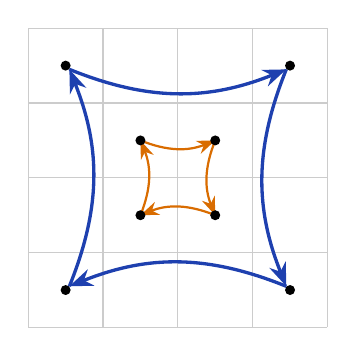
\begin{tikzpicture}[scale=0.95,>=Stealth,font=\small]
  \foreach \x in {0,1,2,3,4} \draw[gray!40] (\x,0)--(\x,4);
  \foreach \y in {0,1,2,3,4} \draw[gray!40] (0,\y)--(4,\y);
  % corner 4-cycle
  \draw[->,very thick,accent] (0.55,3.45) to[bend right=22] (3.45,3.45);
  \draw[->,very thick,accent] (3.45,3.45) to[bend right=22] (3.45,0.55);
  \draw[->,very thick,accent] (3.45,0.55) to[bend right=22] (0.55,0.55);
  \draw[->,very thick,accent] (0.55,0.55) to[bend right=22] (0.55,3.45);
  % inner 4-cycle
  \draw[->,thick,orange!85!black] (1.5,2.5) to[bend right=22] (2.5,2.5);
  \draw[->,thick,orange!85!black] (2.5,2.5) to[bend right=22] (2.5,1.5);
  \draw[->,thick,orange!85!black] (2.5,1.5) to[bend right=22] (1.5,1.5);
  \draw[->,thick,orange!85!black] (1.5,1.5) to[bend right=22] (1.5,2.5);
  \foreach \c in {(0.5,3.5),(3.5,3.5),(3.5,0.5),(0.5,0.5),(1.5,2.5),(2.5,2.5),(2.5,1.5),(1.5,1.5)}
     \fill \c circle (1.9pt);
\end{tikzpicture}\\[2pt]
{\small 图 1\ \ $n=4$：旋转把四个角点串成一个\textbf{4-循环}（蓝），中心的 $2\times2$ 又是另一个 4-循环（橙）。}
\end{center}

\section*{五、致命点：用“二元对换”去做“四元循环”}

\begin{center}
\renewcommand{\arraystretch}{1.35}
\begin{tabular}{@{}p{6.3cm}p{6.3cm}@{}}
\toprule
\textbf{转置 $T$：$(i,j)\mapsto(j,i)$} & \textbf{旋转 $R$：$(i,j)\mapsto(n{-}1{-}j,\,i)$}\\
\midrule
$T^{2}=I$（对合） & $R^{2}\neq I,\ R^{4}=I$\\
轨道是 \textbf{2-循环} & 轨道是 \textbf{4-循环}\\
用一次 \texttt{swap} 就够 & 必须用一个临时变量做 \textbf{4 元轮换}\\
遍历上三角（如 $j<i$） & 需按轨道整圈搬运\\
\bottomrule
\end{tabular}
\end{center}

\begin{center}
\begin{tikzpicture}[>=Stealth,font=\small]
  \node[draw,rounded corners,fill=blue!8,minimum width=1.5cm,minimum height=0.8cm] (a) at (0,0) {$(i,j)$};
  \node[draw,rounded corners,fill=blue!8,minimum width=1.5cm,minimum height=0.8cm] (b) at (2.6,0) {$(j,i)$};
  \draw[<->,thick,accent] (a) to[bend left=20] (b);
  \draw[<->,thick,accent] (a) to[bend right=20] (b);
  \node at (1.3,-1.05) {转置：2-循环};
\end{tikzpicture}
\hspace{1.6cm}
\begin{tikzpicture}[>=Stealth,font=\small]
  \node[draw,rounded corners,fill=orange!10,minimum width=1.7cm,minimum height=0.75cm] (p0) at (0,0) {$p$};
  \node[draw,rounded corners,fill=orange!10,minimum width=1.7cm,minimum height=0.75cm] (p1) at (2.1,1.25) {$Rp$};
  \node[draw,rounded corners,fill=orange!10,minimum width=1.7cm,minimum height=0.75cm] (p2) at (4.2,0) {$R^{2}p$};
  \node[draw,rounded corners,fill=orange!10,minimum width=1.7cm,minimum height=0.75cm] (p3) at (2.1,-1.25) {$R^{3}p$};
  \draw[->,thick,orange!85!black] (p0)--(p1);
  \draw[->,thick,orange!85!black] (p1)--(p2);
  \draw[->,thick,orange!85!black] (p2)--(p3);
  \draw[->,thick,orange!85!black] (p3)--(p0);
  \node at (2.1,-2.15) {旋转：4-循环};
\end{tikzpicture}\\[2pt]
{\small 图 2\ \ 同为“搬动格子”，转置只需对换，旋转必须整圈轮换——这就是本题程序错误的根源。}
\end{center}

\textbf{区域重叠：}外层 $i$ 取遍所有行，内层 $j< n/2$，所以它只枚举了\textbf{左} $\lfloor n/2\rfloor$ 列（蓝色区域 $L$）。但每次交换还同时写\textbf{下} $\lfloor n/2\rfloor$ 行（橙色区域 $B$）。于是
\[
L\cap B=\text{左下 } \Bigl\lfloor \tfrac n2\Bigr\rfloor\times\Bigl\lfloor \tfrac n2\Bigr\rfloor \text{ 块（紫色 }O\text{）}
\]
里的格子，既当“左格”又被当“右格”，会被交换两次，结果\textbf{依赖执行顺序}。这就不是一次“齐整”的置换，更不可能是纯旋转。

\begin{warnbox}
\textbf{用行列式一击致命（以 $n=3$ 为例）：}交换次数 $k=n\lfloor n/2\rfloor$，故 $\det P=(-1)^{k}$。取 $n=3$：$k=3$ 为奇数，$\det P=-1$。而 $n=3$ 的 90\textdegree{} 旋转把 8 个非中心格排成\textbf{两个 4-循环}，作为置换其符号为 $(-1)^{3}\cdot(-1)^{3}=+1$。二者反号，所以这段程序\textbf{不可能}是（$n=3$ 的）90\textdegree{} 旋转。（更本质的理由仍是：二元对换的“阶”与四元循环不匹配。）
\end{warnbox}

\section*{六、程序实际做了什么：精确追踪}

用原程序实测（与逐句模拟一致）得到：

\begin{center}
\renewcommand{\arraystretch}{1.28}
\begin{tabular}{@{}c l@{}}
\toprule
$n$ & 输出（每行以 “\#\ ” 结尾）\\
\midrule
2 & \texttt{2 1 \# 3 0 \#}\\
3 & \texttt{6 1 2 \# 7 4 5 \# 8 3 0 \#}\\
4 & \texttt{12 8 2 3 \# 13 9 6 7 \# 14 10 5 4 \# 15 11 1 0 \#}\\
5 & \texttt{20 15 2 3 4 \# 21 16 7 8 9 \# 22 17 12 13 14 \#}\\
  & \texttt{23 18 11 6 5 \# 24 19 10 1 0 \#}\\
6 & \texttt{30 24 18 3 4 5 \# 31 25 19 9 10 11 \# 32 26 20 15 16 17 \#}\\
  & \texttt{33 27 21 14 13 12 \# 34 28 22 8 7 6 \# 35 29 23 2 1 0 \#}\\
\bottomrule
\end{tabular}
\end{center}

当 $n$ 为\textbf{偶数}（记 $m=n/2$）时，最终矩阵 $F$ 恰可写成清爽的“三块拼接”：
\[
\boxed{
\begin{aligned}
F_{ij}&=A_{\,n-1-j,\ i}, && 0\le j<m;\\[2pt]
F_{ij}&=A_{ij}, && j\ge m,\ i<m;\\[2pt]
F_{ij}&=A_{\,n-1-i,\ n-1-j}, && i\ge m,\ j\ge m.
\end{aligned}}
\]
用分块的话说：
\begin{itemize}
\item $F$ 的\textbf{左半}（左 $m$ 列）$=$ 把 $A$ 的\textbf{下半}上下翻转后转置；
\item $F$ 的\textbf{右上块} $=$ $A$ 的右上块（原样不动）；
\item $F$ 的\textbf{右下块} $=$ $A$ 的左上块旋转 180\textdegree。
\end{itemize}

\begin{center}
\begin{minipage}{0.96\linewidth}
\centering
{\footnotesize
\MatAfour \hspace{0.5cm}$\longrightarrow$\hspace{0.5cm}\MatFfour}\\[2pt]
{\small 图 3\ \ $n=4$：左 $A$、右 $F$；只有左半被搬动，右上不动，右下为左上块的 180\textdegree。}
\end{minipage}
\end{center}

$n=6$ 时同样如此（左图 $A$，右图 $F$）：
\begin{center}
\begin{minipage}{0.96\linewidth}
\centering
{\footnotesize
\MatA \hspace{0.35cm}$\longrightarrow$\hspace{0.35cm}\MatF}\\[2pt]
{\small 图 4\ \ $n=6$：蓝色左半来自 $A$ 的下半（翻转为行、再转置成列），右侧为“右上原样、右下 180\textdegree”。}
\end{minipage}
\end{center}

注意 $n$ 为\textbf{奇数}时，重叠块不是方阵，三段公式不再成立，只能逐格追踪（上表已给出 $n=3,5$ 的实测输出）。

\section*{七、修改方案与线性代数小结}

\begin{keybox}
\textbf{若原意是“转置”：}把伙伴改成 $a[j][i]$，并只遍历上三角，即可（转置是对合，二元对换天然合适）。正确写法：
\end{keybox}
\begin{lstlisting}
for (i = 0; i < n; i++)
    for (j = 0; j < i; j++) {      /* 只走上三角以下 */
        temp = a[i][j];
        a[i][j] = a[j][i];
        a[j][i] = temp;
    }
\end{lstlisting}
\begin{keybox}
\textbf{若原意是“旋转 90\textdegree”：}必须做 4 元轮换（一个临时变量沿 4-循环搬运），或干脆另开数组
\[
\text{new}[\,i\,][\,j\,]=\text{old}[\,n-1-j\,][\,i\,],
\]
也可分解为“转置 $+$ 逐行反转”两个反射的复合（$\det=(-1)(-1)=+1$，与旋转一致）。
\end{keybox}

\begin{warnbox}
\textbf{线性代数三句话总结：}
\begin{enumerate}
\item 数组 $=$ 矩阵 $A$；把元素互换 $=$ 对 $\operatorname{vec}(A)$ 左乘\textbf{置换矩阵}（正交阵，$\det=\pm1$）。
\item 配对 $(i,j)\mapsto(n{-}1{-}j,i)$ 是\textbf{90\textdegree 旋转 $R$}，$R^{4}=I$，轨道是 4-循环；而二元对换只有 2 阶——\textbf{用错工具}。
\item 再加上扫描区与写入区重叠于左下块，同一格被反复交换，最终 $P$ 既非转置也非旋转；$n=3$ 时 $\det P=-1$ 即可否定“旋转”之说。
\end{enumerate}
\end{warnbox}

\vfill
\begin{center}
{\small\color{gray} 结论：这是一道“概念错配”型阅读题——认清“转置是 2-循环、旋转是 4-循环”，比死记输出更重要。}
\end{center}

\newpage
\section*{附：$n=4$ 时怎样写成 $Ax=b$}

取 $n=4$，把矩阵\textbf{按行优先拉直成 16 维向量}，并以“源矩阵 $A$ 的元素”为未知量 $x$、以“输出矩阵 $F$ 的元素”为右端 $b$：
\[
x=\operatorname{vec}(A)=(a_{11},a_{12},a_{13},a_{14},a_{21},\dots,a_{44})^{T}=(x_0,x_1,\dots,x_{15})^{T},
\]
\[
b=\operatorname{vec}(F)=(b_0,b_1,\dots,b_{15})^{T},\qquad b_k=F\!\left(\left\lfloor k/4\right\rfloor,\ k\bmod 4\right).
\]

\textbf{第一步：把 8 次交换写成对换阵。}$n/2=2$，循环共 $4\times2=8$ 次交换；换算成扁平下标为
\[
0\!\leftrightarrow\!12,\quad 1\!\leftrightarrow\!8,\quad 4\!\leftrightarrow\!13,\quad 5\!\leftrightarrow\!9,\quad
8\!\leftrightarrow\!14,\quad 9\!\leftrightarrow\!10,\quad 12\!\leftrightarrow\!15,\quad 13\!\leftrightarrow\!11 .
\]
每次交换对应一个对换矩阵 $T_s$（单位阵交换两行），整段程序即
\[
b=P\,x,\qquad P=T_{8}T_{7}\cdots T_{1}.
\]
注意这些对换\textbf{并不互不相交}：下标 $8,9,12,13$ 各被用两次，所以连乘后并\\不是 8 个 2-循环，而是合并成 3-循环：
\[
(0\ \ 15\ \ 12),\quad (1\ \ 14\ \ 8),\quad (4\ \ 11\ \ 13),\quad (5\ \ 10\ \ 9),\quad 2,3,6,7\ \text{不动}.
\]

\textbf{第二步：展开成 16 个方程。}$P$ 每行每列恰有一个 1，于是
\[
\begin{aligned}
b_0&=x_{12}, & b_1&=x_{8}, & b_2&=x_{2}, & b_3&=x_{3},\\
b_4&=x_{13}, & b_5&=x_{9}, & b_6&=x_{6}, & b_7&=x_{7},\\
b_8&=x_{14}, & b_9&=x_{10}, & b_{10}&=x_{5}, & b_{11}&=x_{4},\\
b_{12}&=x_{15}, & b_{13}&=x_{11}, & b_{14}&=x_{1}, & b_{15}&=x_{0}.
\end{aligned}
\]
这就是本题的“$Ax=b$”形态（此处系数矩阵 $A\equiv P$）。它的非零元位置如下图（横轴为源下标 $m$，纵轴为目标下标 $k$）：

\begin{center}
\begin{tikzpicture}[scale=0.29]
  \draw[gray!30,step=1] (0,0) grid (16,-16);
  \foreach \k/\m in {0/12,1/8,2/2,3/3,4/13,5/9,6/6,7/7,8/14,9/10,10/5,11/4,12/15,13/11,14/1,15/0}{
     \fill[accent] (\m+0.5,-\k-0.5) circle (0.30);
  }
  \node[font=\scriptsize] at (8,0.85){列 $=$ 源下标 $m$};
  \node[font=\scriptsize,rotate=90] at (-0.95,-8){行 $=$ 目标下标 $k$};
\end{tikzpicture}\\[2pt]
{\small 图 5\ \ $16\times16$ 置换矩阵 $P$ 的非零元：每行每列一个点，故 $P$ 可逆且 $P^{-1}=P^{T}$。}
\end{center}

\textbf{第三步：看清它的块结构。}按四条 3-循环重排坐标，$P$ 相似于分块对角
\[
P\ \sim\ \operatorname{diag}(C,C,C,C,1,1,1,1),\qquad
C=\begin{pmatrix}0&0&1\\[1pt]1&0&0\\[1pt]0&1&0\end{pmatrix},\qquad C^{3}=I .
\]
于是
\[
\det P=(\det C)^{4}=1,\qquad P^{-1}=P^{T},
\]
方程组有唯一解 $x=P^{T}b$；但因为 $P$ 是置换矩阵，\textbf{根本不用高斯消元}，按上表逐行“对号入座”即可。

\begin{warnbox}
\textbf{关键对照：}真正的 90\textdegree{} 旋转在 $n=4$ 时应分解为\textbf{四个 4-循环}（每块是 $C_4$，$C_4^{4}=I$）；而本题实际得到的是\textbf{四个 3-循环}。循环长度从 4 变成 3，再一次用线性代数（置换的循环型）证明：这段程序不是旋转。若把未知量取成输出、右端取成输入，则写成 $P\,x=b$；两种写法只差一个转置，本质是同一个方程组。
\end{warnbox}

\end{document}
